\section{Tests for CI} Providing a set of regression tests for the CI pipeline is clearly good practice since they will be executed with every change provided to the remote repository and make sure that if any of those changes will affect the functionality of the tested code the pipeline will fail and the code with defects will not be deployed. Moreover, tests will tell the developer exactly what unit was affected by their changes and require a fix.


\subsection{Vitest} Vite is a frontend build tool used for the BI-DBS frontend. Vitest is a unit test framework built on top of Vite. It is a suitable tool for implementing tests in the project like the BI-DBS frontend which uses Vite. Vitest cares a lot about performance and speed, which makes it a good choice for tests that will be a part of CI pipeline. \cite{vitest}

\subsection{Tests} The authorization module is composed of four main services which I have implemented for authentication and authorization processes including additional features like a refreshing of token and logging out. Therefore I have created unit tests for the functionalities of those services.\\


\paragraph*{Generating the access token service.} The process of getting the access token enables the application to log in the user on the frontend after an authorization server has successfully authorized the user and provided the client with the authorization code. This service is focused on exchanging that code for an access token with the backend and handling the response from the server.


\paragraph*{Test cases for the token generating service} 
\begin{itemize}
    \item \emph{Positive scenario:} 
        \begin{itemize}
            \item \emph{Conditions:} A valid token is successfully returned in the valid response.
            \item \emph{Expected result:} User was successfully authorized.
        \end{itemize}
    \item \emph{Negative scenario} 
        \begin{itemize}
            \item \emph{Conditions:} An invalid token is successfully returned in the valid response.
            \item \emph{Expected result.} The errors from parsing the token are successfully handled and the user was not authorized.
        \end{itemize}
    \item \emph{Negative scenario.} 
        \begin{itemize}
            \item \emph{Conditions:} The request for getting the access token fails.
            \item \emph{Expected result:} The errors from the request are successfully handled and the user was not authorized.
        \end{itemize}
\end{itemize}

\

\paragraph*{Refreshing the access token service.} Refreshing process prolongs the authorized status for a user without the need of submitting credentials, which is implemented by exchanging the refresh token and current access token for the new access token with the backend. 


\paragraph*{Test cases for the token refreshing service} 
\begin{itemize}
    \item \emph{Positive scenario:} 
        \begin{itemize}
            \item \emph{Conditions:} User is authorized and the request for refreshing the access token succeeded and the server returned a new valid access token.
            \item \emph{Expected result:} The authorization time for a user was prolonged to the expiration time of the newly received access token.
        \end{itemize}
    \item \emph{Negative scenario} 
        \begin{itemize}
            \item \emph{Conditions:} User is authorized and the request for refreshing the access token succeeded but returned an invalid token.
            \item \emph{Expected result.} The errors from parsing the token are successfully handled and the user was logged out.
        \end{itemize}
    \item \emph{Negative scenario.} 
        \begin{itemize}
            \item \emph{Conditions:} The request for refreshing the access token fails.
            \item \emph{Expected result:} The errors from the request are successfully handled and the user was not logged out.
        \end{itemize}
\end{itemize}

\


\paragraph*{Rejecting the access token.}The process of logging out is implemented as a rejection of a token which includes removing all of the user's data from the user's store along with permissions to access the components which require authorization.

\paragraph*{Test cases for the token rejecting service} 
\begin{itemize}
    \item \emph{Positive scenario:} 
        \begin{itemize}
            \item \emph{Conditions:} User is authorized and the request for rejecting the access token succeeded.
            \item \emph{Expected result:} User was successfully logged out.
        \end{itemize}
\end{itemize}

\noindent Negative scenario test for the rejection of the token does not have to be provided as the service behavior as for the positive scenario.

\


\paragraph*{Authorization service.} The services described above also need some additional functionalities like parsing the data from the request and preparing the URL for communication with the authorization server which are implemented in the authorization service with both positive and negative scenarios. 


\paragraph*{Test cases for the authorization service} 
\begin{itemize}
    \item \emph{Positive scenario:} 
        \begin{itemize}
            \item \emph{Conditions:} The frontend calls the function to create an URL to initiate an authorization process by sending a request to the authorization server,
            \item \emph{Expected result:} The URL is valid.
        \end{itemize}
    \item \emph{Positive scenario.} This scenario is used for the implementation of four tests for each user's role: admin, guarantor, teacher and student
        \begin{itemize}
            \item \emph{Conditions:} The frontend calls the function to process the access JWT token it got from the server for authorization of a user with a certain role.
            \item \emph{Expected result.} Successfully parsed the token and the data in the user store matches the user's identity sent in a token including the role.
        \end{itemize}
\end{itemize}

\ 

\paragraph*{The results of unit testing.} Frankly speaking, in the beginning I underestimated the importance of the unit tests implementation as I was very confident about my code as it was structured and clear for me to work correctly. Moreover, multiple times I have successfully tested all the functionalities manually myself.\\
Unexpectedly, The implementation of the unit tests process helped me to uncover and correct some weaknesses in the implementation of some functions. But most importantly, thanks to the creation of tests with also negative scenarios I have found some unhandled errors and was able to test the implementation in the various conditions.\\
The full set of tests is added to the CI pipeline and executed by every change pushed to the repository. The duration of tests as you can see in Figure 6.1 is less than four seconds, which is a remarkably good result.

 \

\begin{figure}[h]
\centering
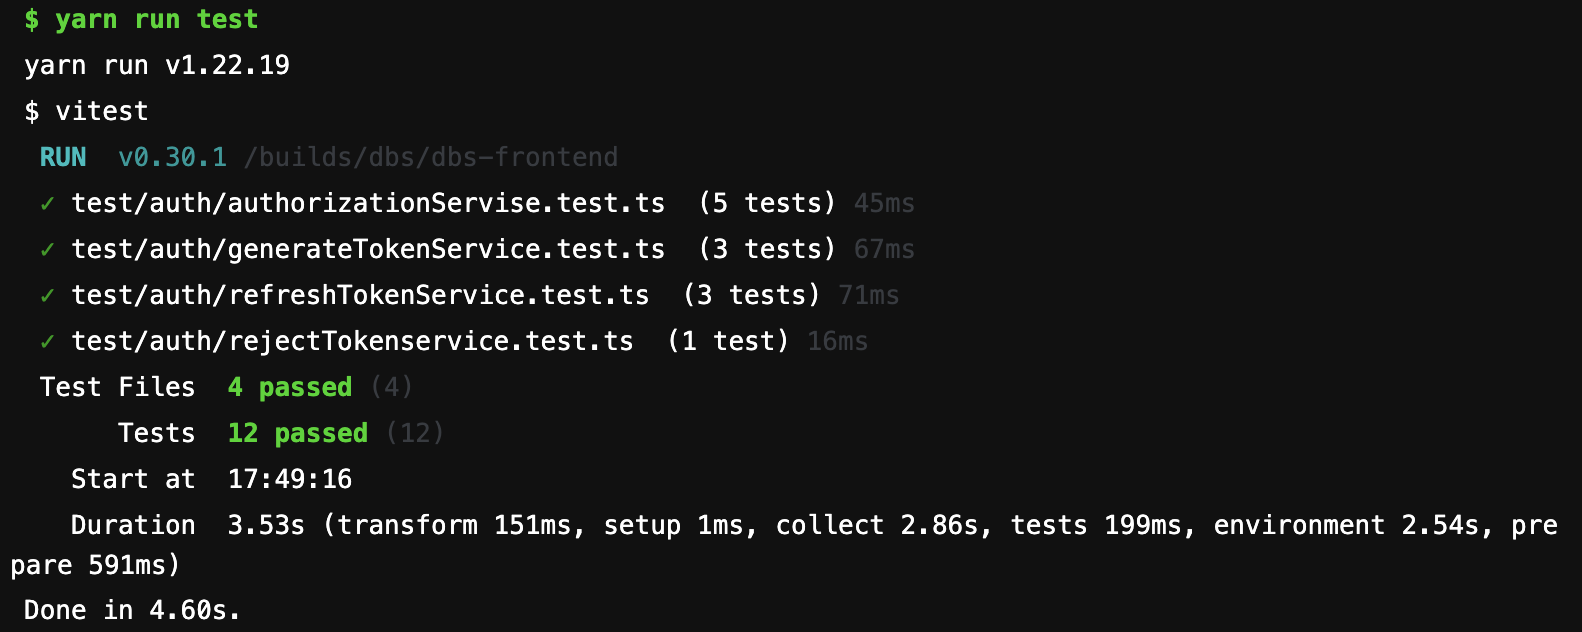
\includegraphics[scale=0.47]{../png/tests.png}
\caption{CI tests}\label{picture:tests}
\end{figure}

